\section{Introduzione}
Lo scopo di questo progetto consiste nella classificazione dell'attività fisica svolta da un individuo effettuando delle misure con una board Arduino Nano 33 BLE Sense posizionata poco sopra la caviglia del soggetto. Per svolgere questa classificazione e in particolare per rilevare le misure sono stati utilizzati i seguenti sensori presenti sulla board:
\begin{itemize}
	\item accelerometro, che ha consentito di ricavare l'accelerazione sui tre assi (x, y e z);
	\item giroscopio, che ha consentito di ricavare la velocità di rotazione sui tre assi (x, y e z);
	\item sensore di temperatura e di umidità, che ha consentito di ricavare la temperatura (in gradi Celsius) e l'umidità.
	\todo{questa riga va tolta?}
\end{itemize}

La metodologia utilizzata per classificare le attività prevede l'utilizzo di una \textit{black box}, che analizza le misure ricevute in ingresso e restituisce la loro classificazione. Questo è stato realizzato mediante una piattaforma di Machine Learning, denominata Edge Impulse, che fornisce delle librerie di classificazione. Le possibili tipologie di attività fisica che possono essere individuate sono: cyclette, fermo, salto della corda e camminata. Analogamente, questa tecnica può essere seguita anche per classificare ulteriori attività fisiche (ad esempio la corsa).

Infine i risultati della classificazione vengono mostrati all'individuo attraverso un'applicazione, che può essere scaricata su un qualsiasi dispositivo e attraverso cui ci si collega al Arduino in modo da poter visualizzare la previsione.

\section{Acquisizione dei dati}
Per poter acquisire i dati con Arduino, è stato necessario sviluppare un firmware apposito che consentisse di eseguire le acquisizioni utilizzando la tecnologia Bluetooth Low Energy (BLE), in cui è stato utilizzato Arduino come \textit{Peripherical}, che trasmette i dati sotto forma di caratteristiche, e l'applicazione come \textit{Central}, che li riceve. \todo{dubbio: o forse i due ruoli sono invertiti?!?}

I dati acquisiti con il BLE, come preannunciato nella sezione precedente, sono: le accelerazioni e le velocità di rotazione entrambe sui tre assi, la temperatura e l'umidità.

Nelle prime acquisizioni delle misure sono stati riscontrati due problemi: il primo riguarda il fatto che il delay tra coppie di misure successive non corrisponde sempre all'incirca a %\SI{15}{\milli\seconds}
(come desiderato) a causa del collegamento BLE, che provoca perdite di tempo; mentre il secondo è relativo alle perdite di campioni  misurati durante l'invio delle misure tramite il BLE. Per questi due motivi all'interno del firmware è stato creato un buffer circolare in modo da poter bufferizzare le acquisizioni da trasmettere nel Bluetooth. In conseguenza a questa modifica si è visto che il delay tra coppie di misure assume sempre valori prossimi a %\SI{15}{\milli\seconds}
e soprattutto che non vengono perse delle acquisizioni perchè vengono mantenute nel buffer.
\todo{ERRORE DA SISTEMARE: non riconosce comando SI}

\todo{inserire anche mutex?}

\todo{mancano dei problemi?}

\section{Edge Impulse}
\todo{I dati acquisisti sono stati caricati su Edge Impulse. Come è stato creato l'impulse. Su cosa lavora. Cosa produce edge impulse. Come son state modificate le finestre. Feature spettrali. Bontà del modello e testing.}

\section{Classificazione delle attività}
\todo{Quali sono i tempi che impiega il firmware. Per passare da una attività all'altra servono circa tot secondi perchè si deve svuotare il buffer.}
Per realizzare la classificazione e poi visualizzarla sull'applicazione è stato sviluppato un ulteriore firmware, al cui interno sono stati creati due thread differenti. Nel primo vengono acquisiti i dati dai sensori fino a quando il buffer non risulta pieno, mentre nel secondo si aggiorna il collegamento BLE in modo da poter trasmettere successivamente la previsione della classificazione. Una volta che il buffer è pieno si estraggono i suoi elementi tramite Digital Signal Processing in modo da convertire il buffer in un segnale, che viene poi passato al classificatore per fare inferenza. La realizzazione concreta della classificazione prevede di richiamare le librerie di Edge Impulse. Infine il risultato della classificazione viene trasmesso tramite una caratteristica su BLE all'applicazione, che mostra a video l'immagine relativa all'attività fisica rilevata. Le possibili schermate visualizzate sull'applicazione si distinguono in base all'attività come mostrato nella figura \ref{fig:attivitafisica}.

\begin{figure}[tbh]
	\centering
	%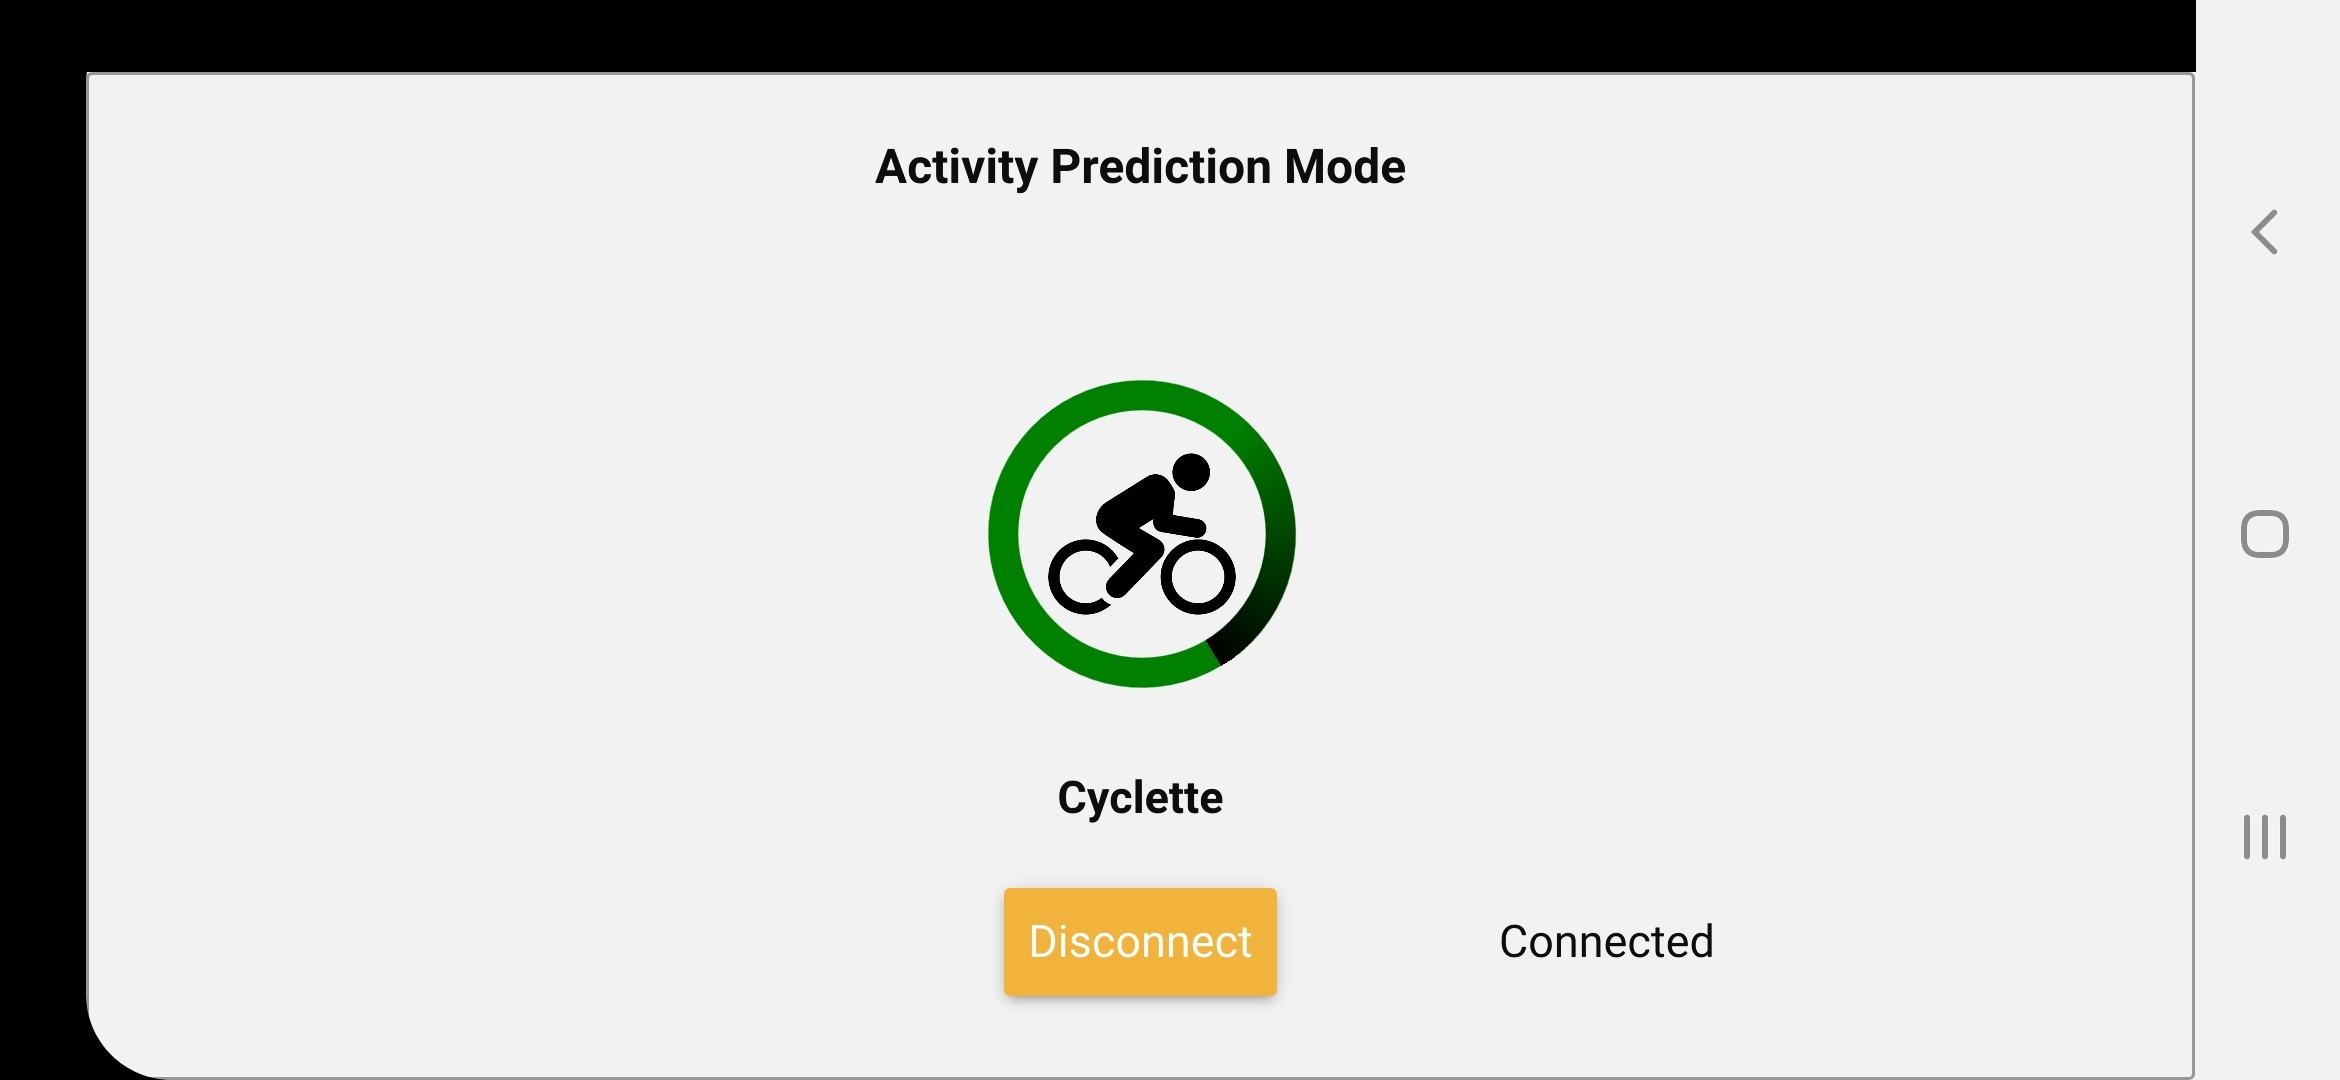
\includegraphics[width=0.4\linewidth]{./ImageFiles/cyclette}
	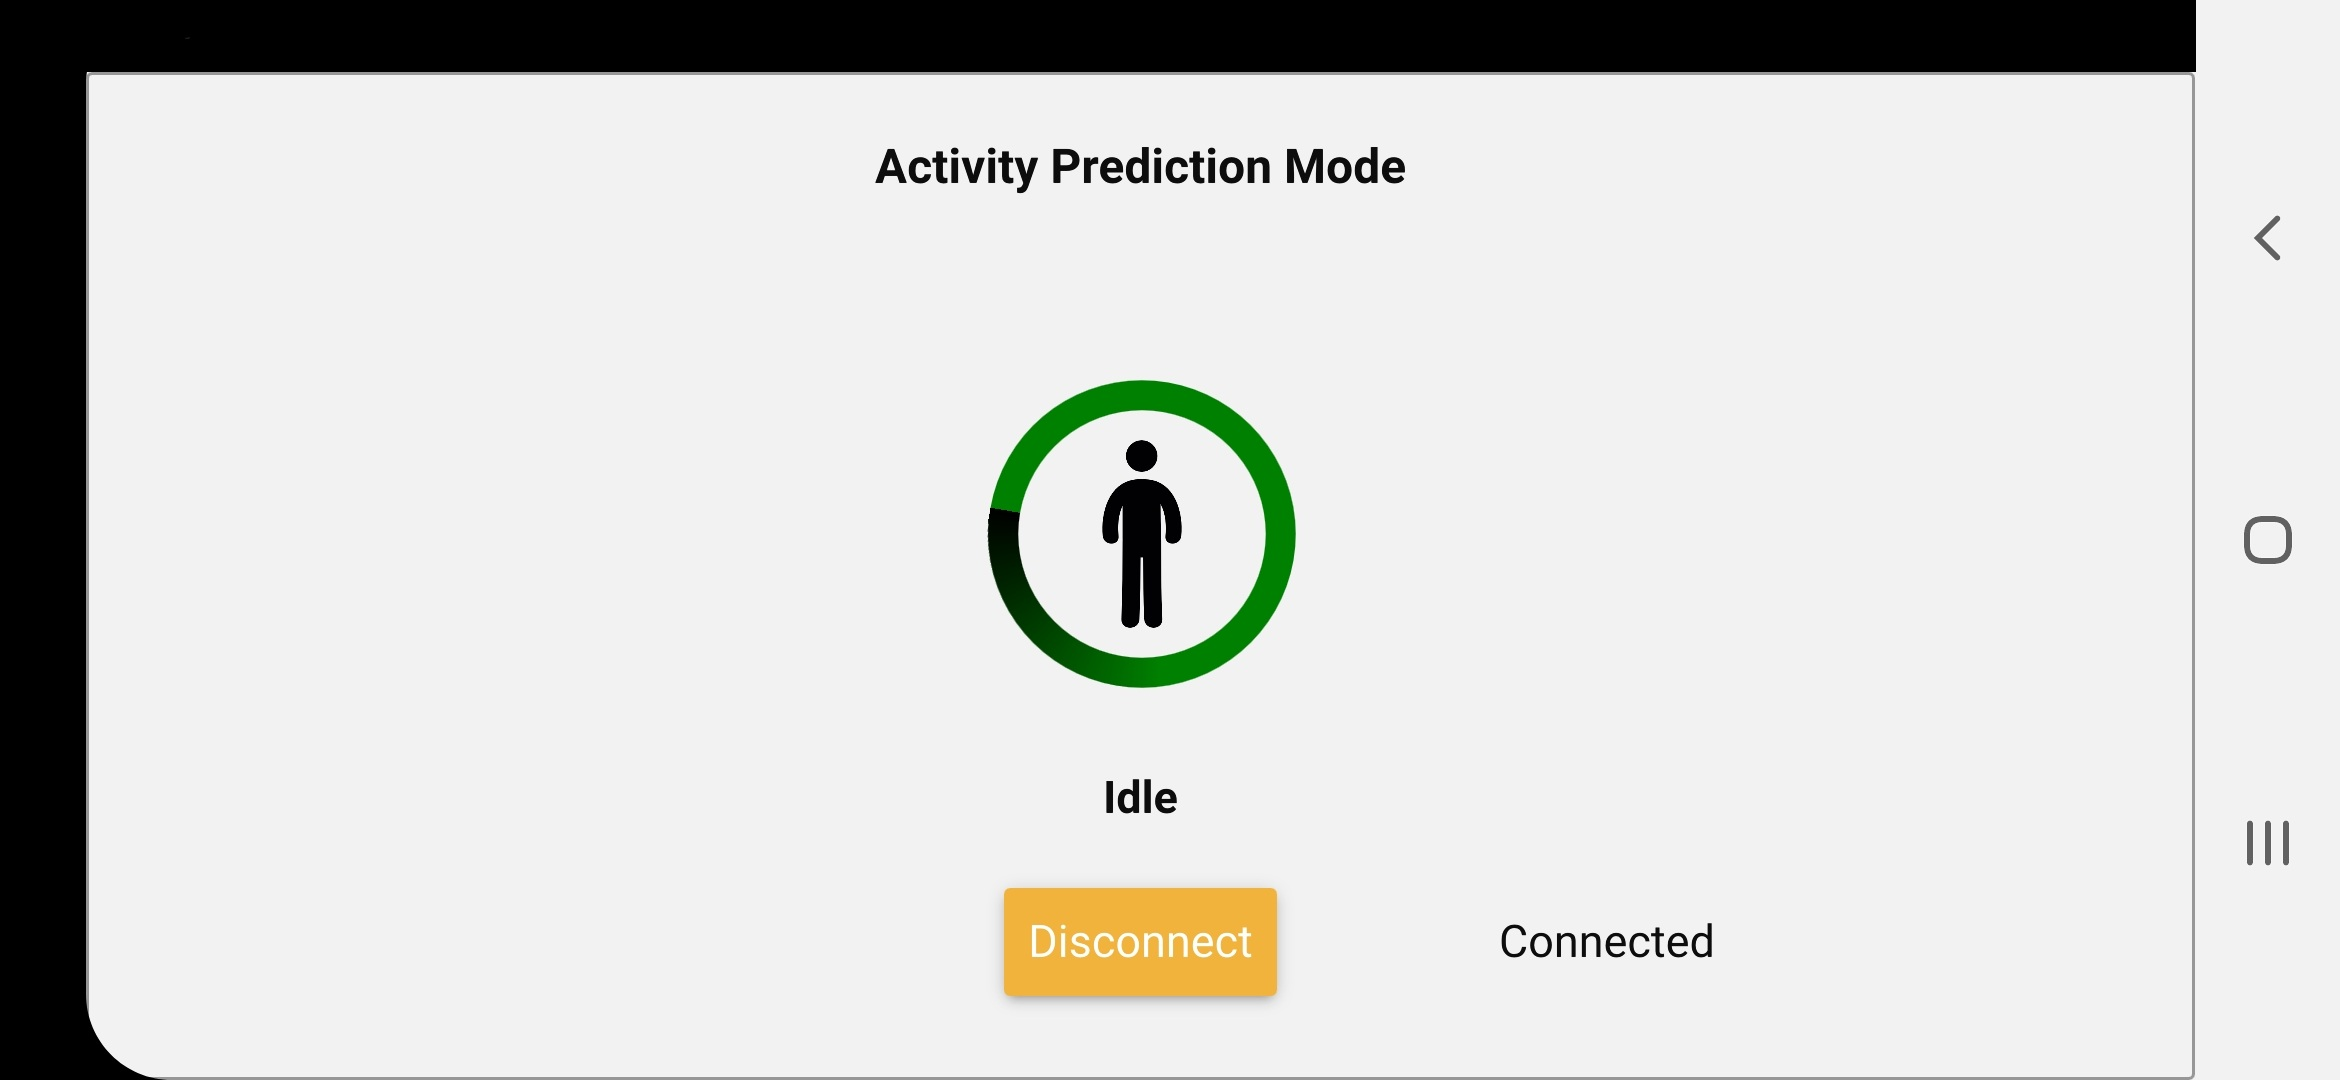
\includegraphics[width=0.4\linewidth]{./ImageFiles/idle}
	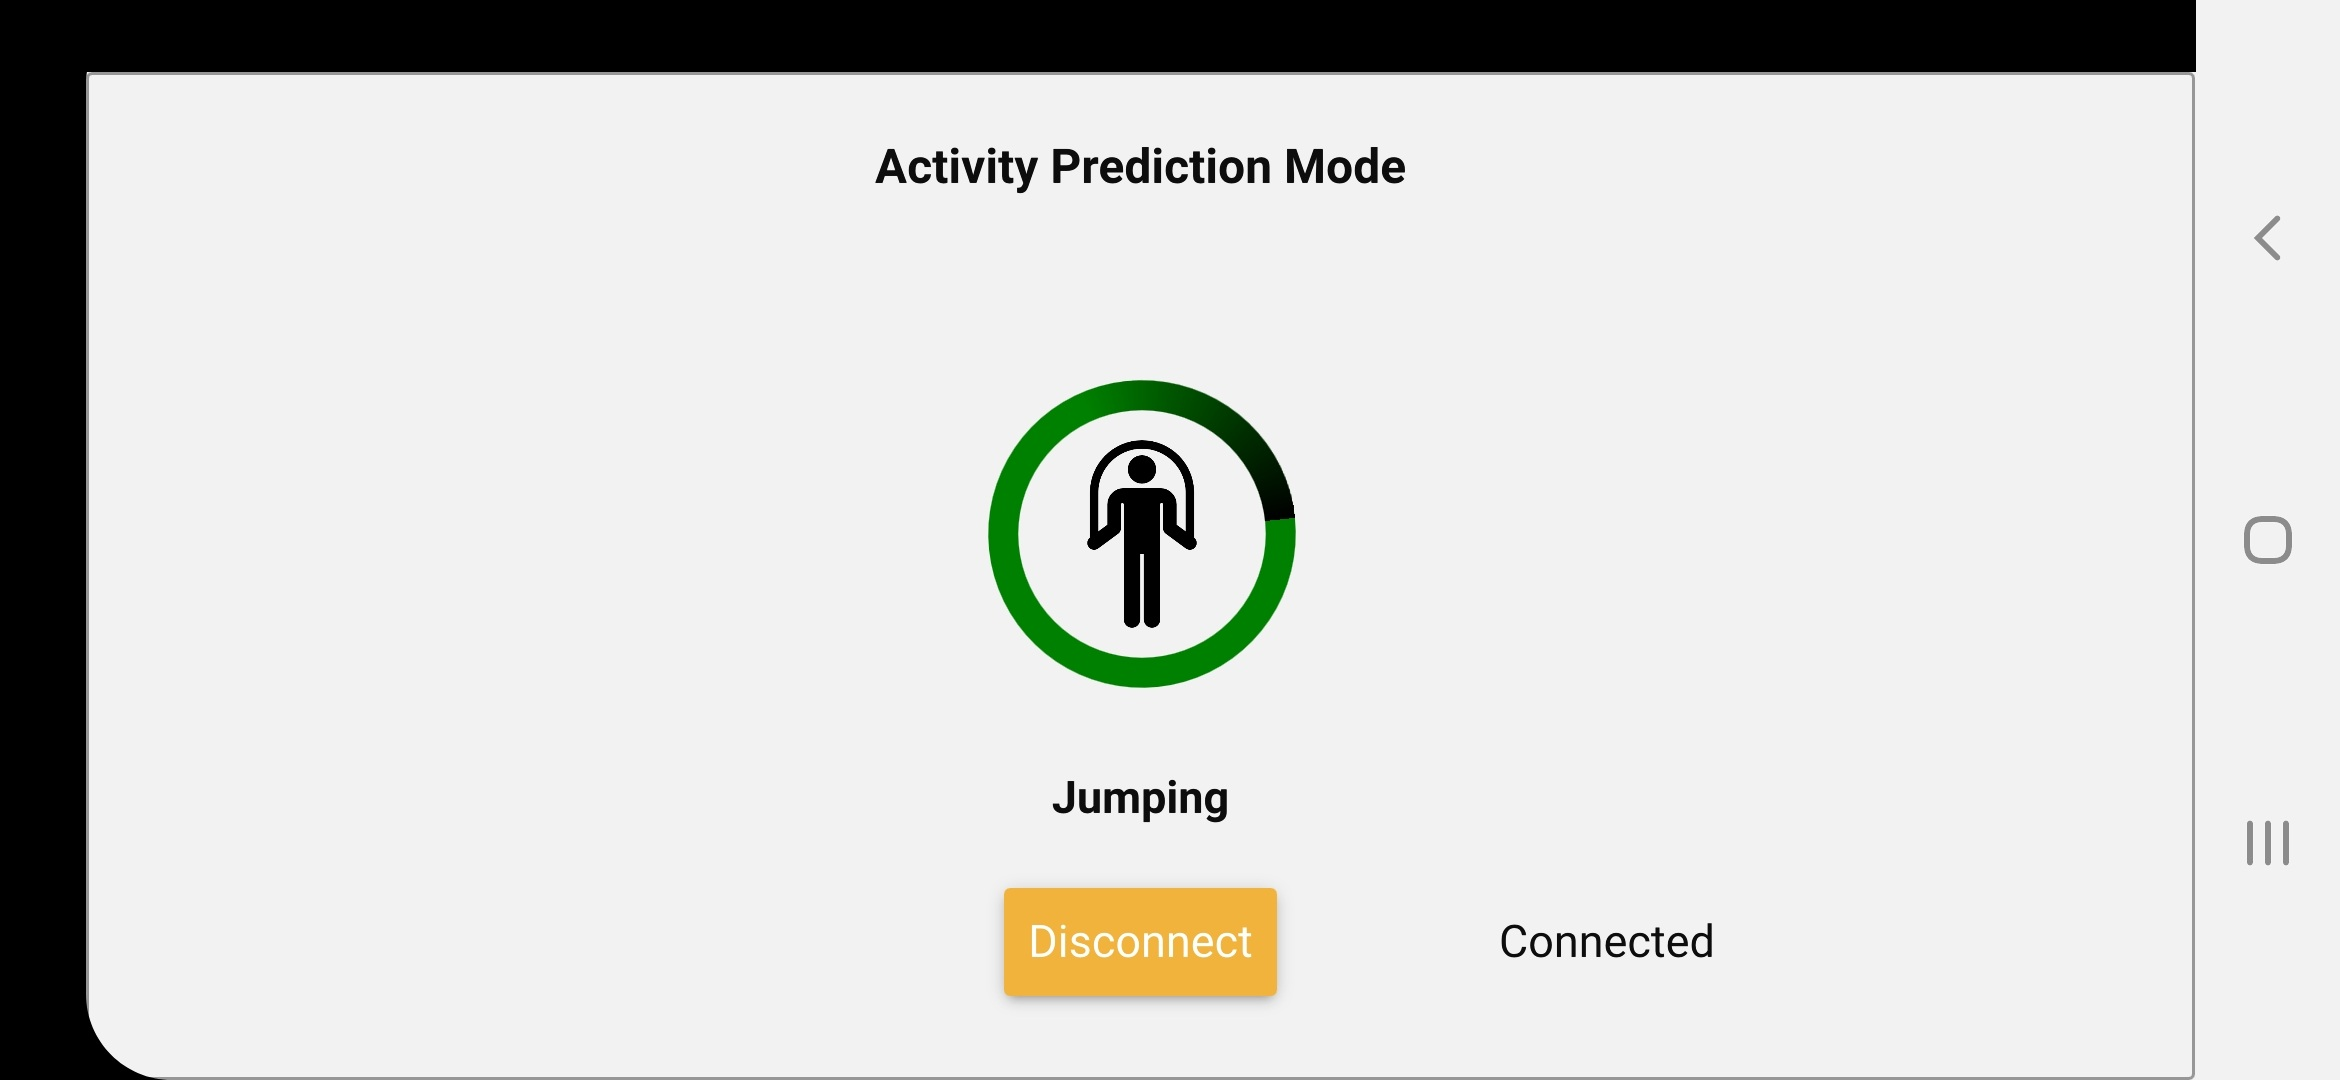
\includegraphics[width=0.4\linewidth]{./ImageFiles/jumping}
	%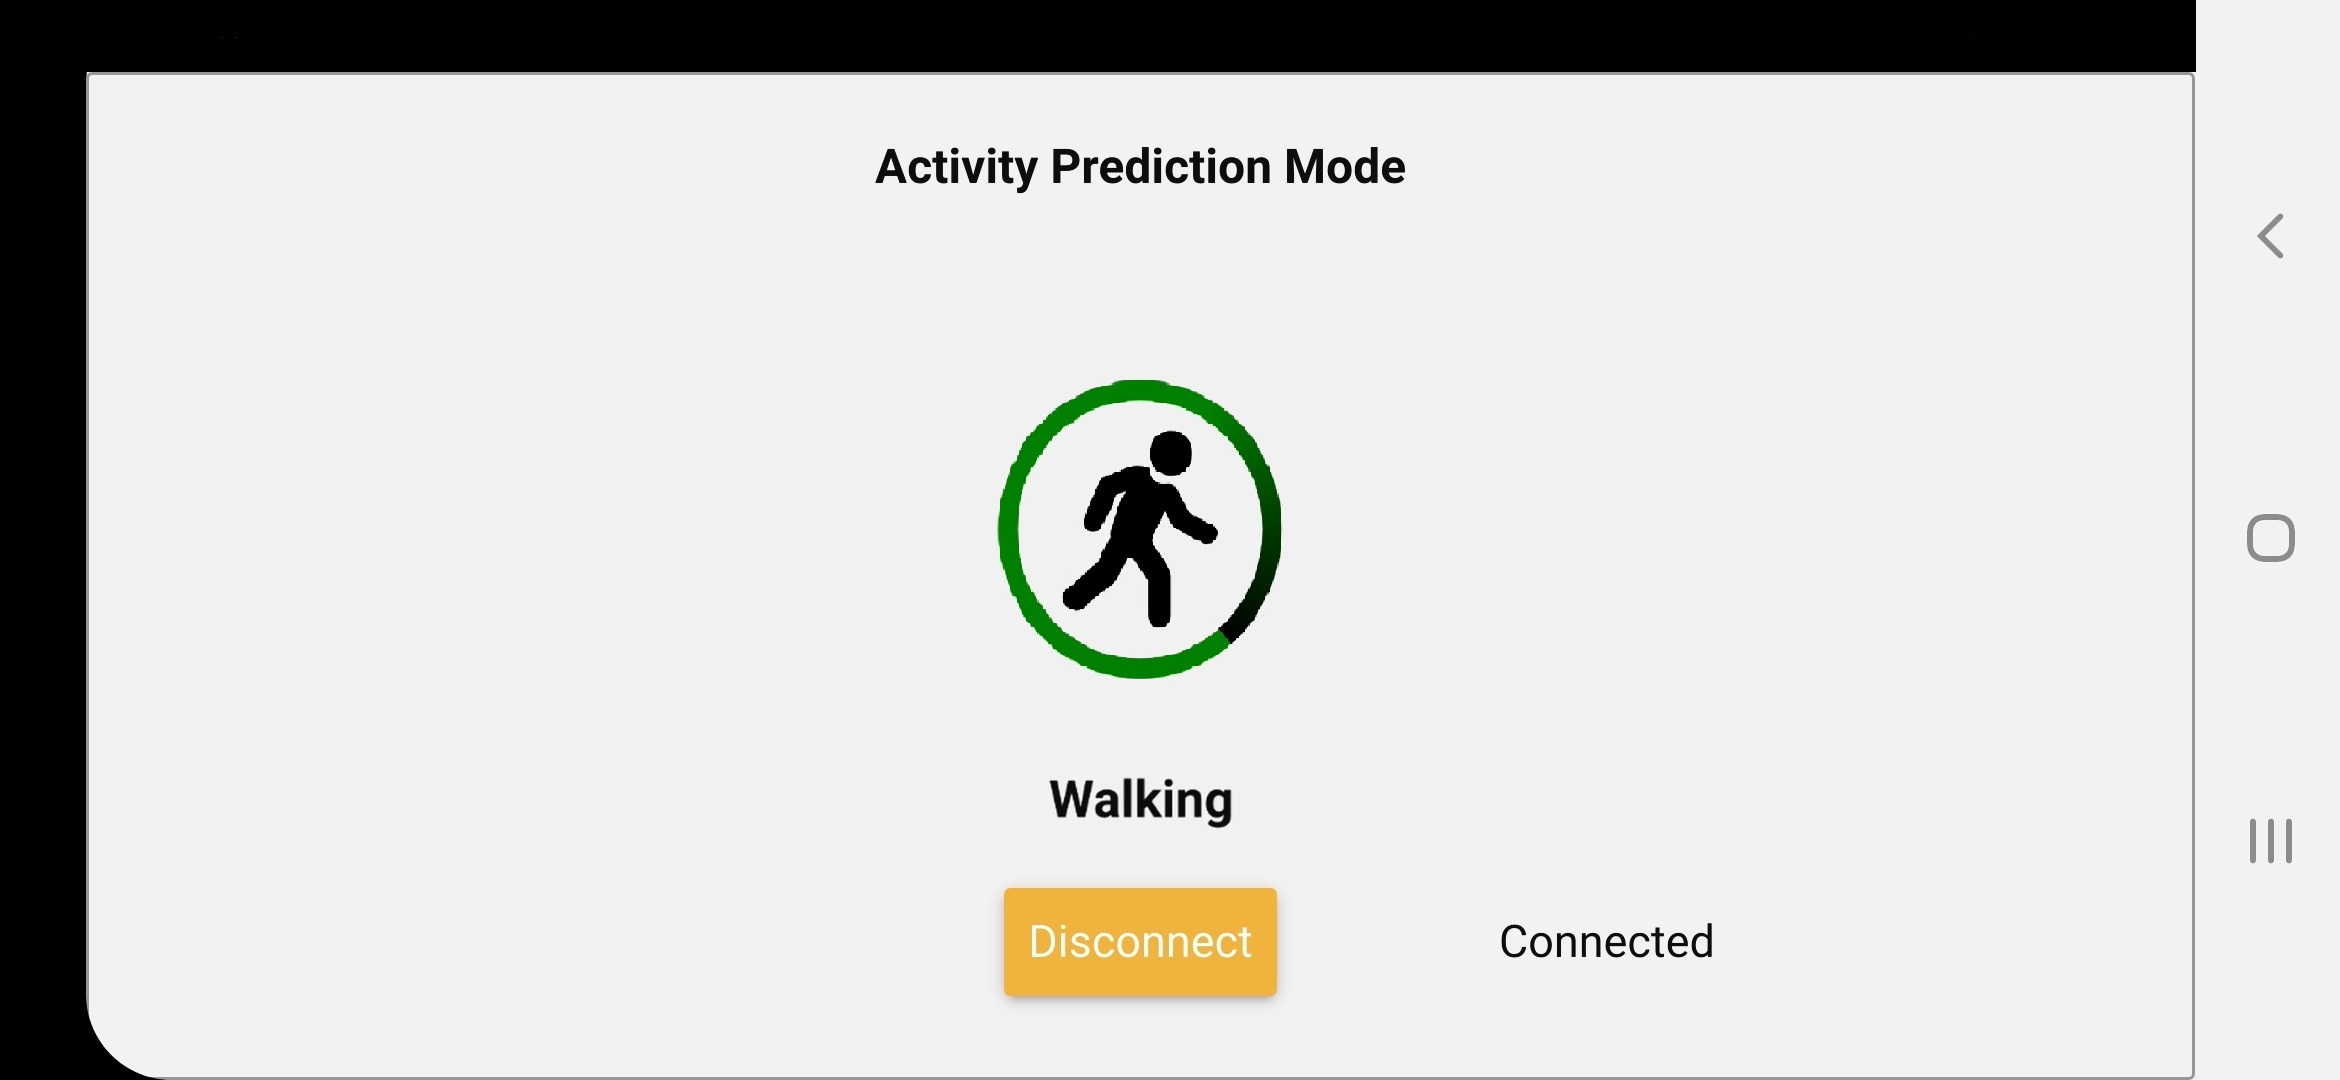
\includegraphics[width=0.4\linewidth]{./ImageFiles/walking}
	\caption{Schermate per le possibili attività: cyclette, fermo in piedi, salto della corda e camminata.}
	\label{fig:attivitafisica}
\end{figure}
\todo{manca schermata cyclette e walking}

Invece nei momenti in cui non si riesce a classificare l'attività in corso in nessuna di quelle possibili si visualizza la schermata della figura \ref{fig:attesa}.

\begin{figure}[tbh]
	\centering
	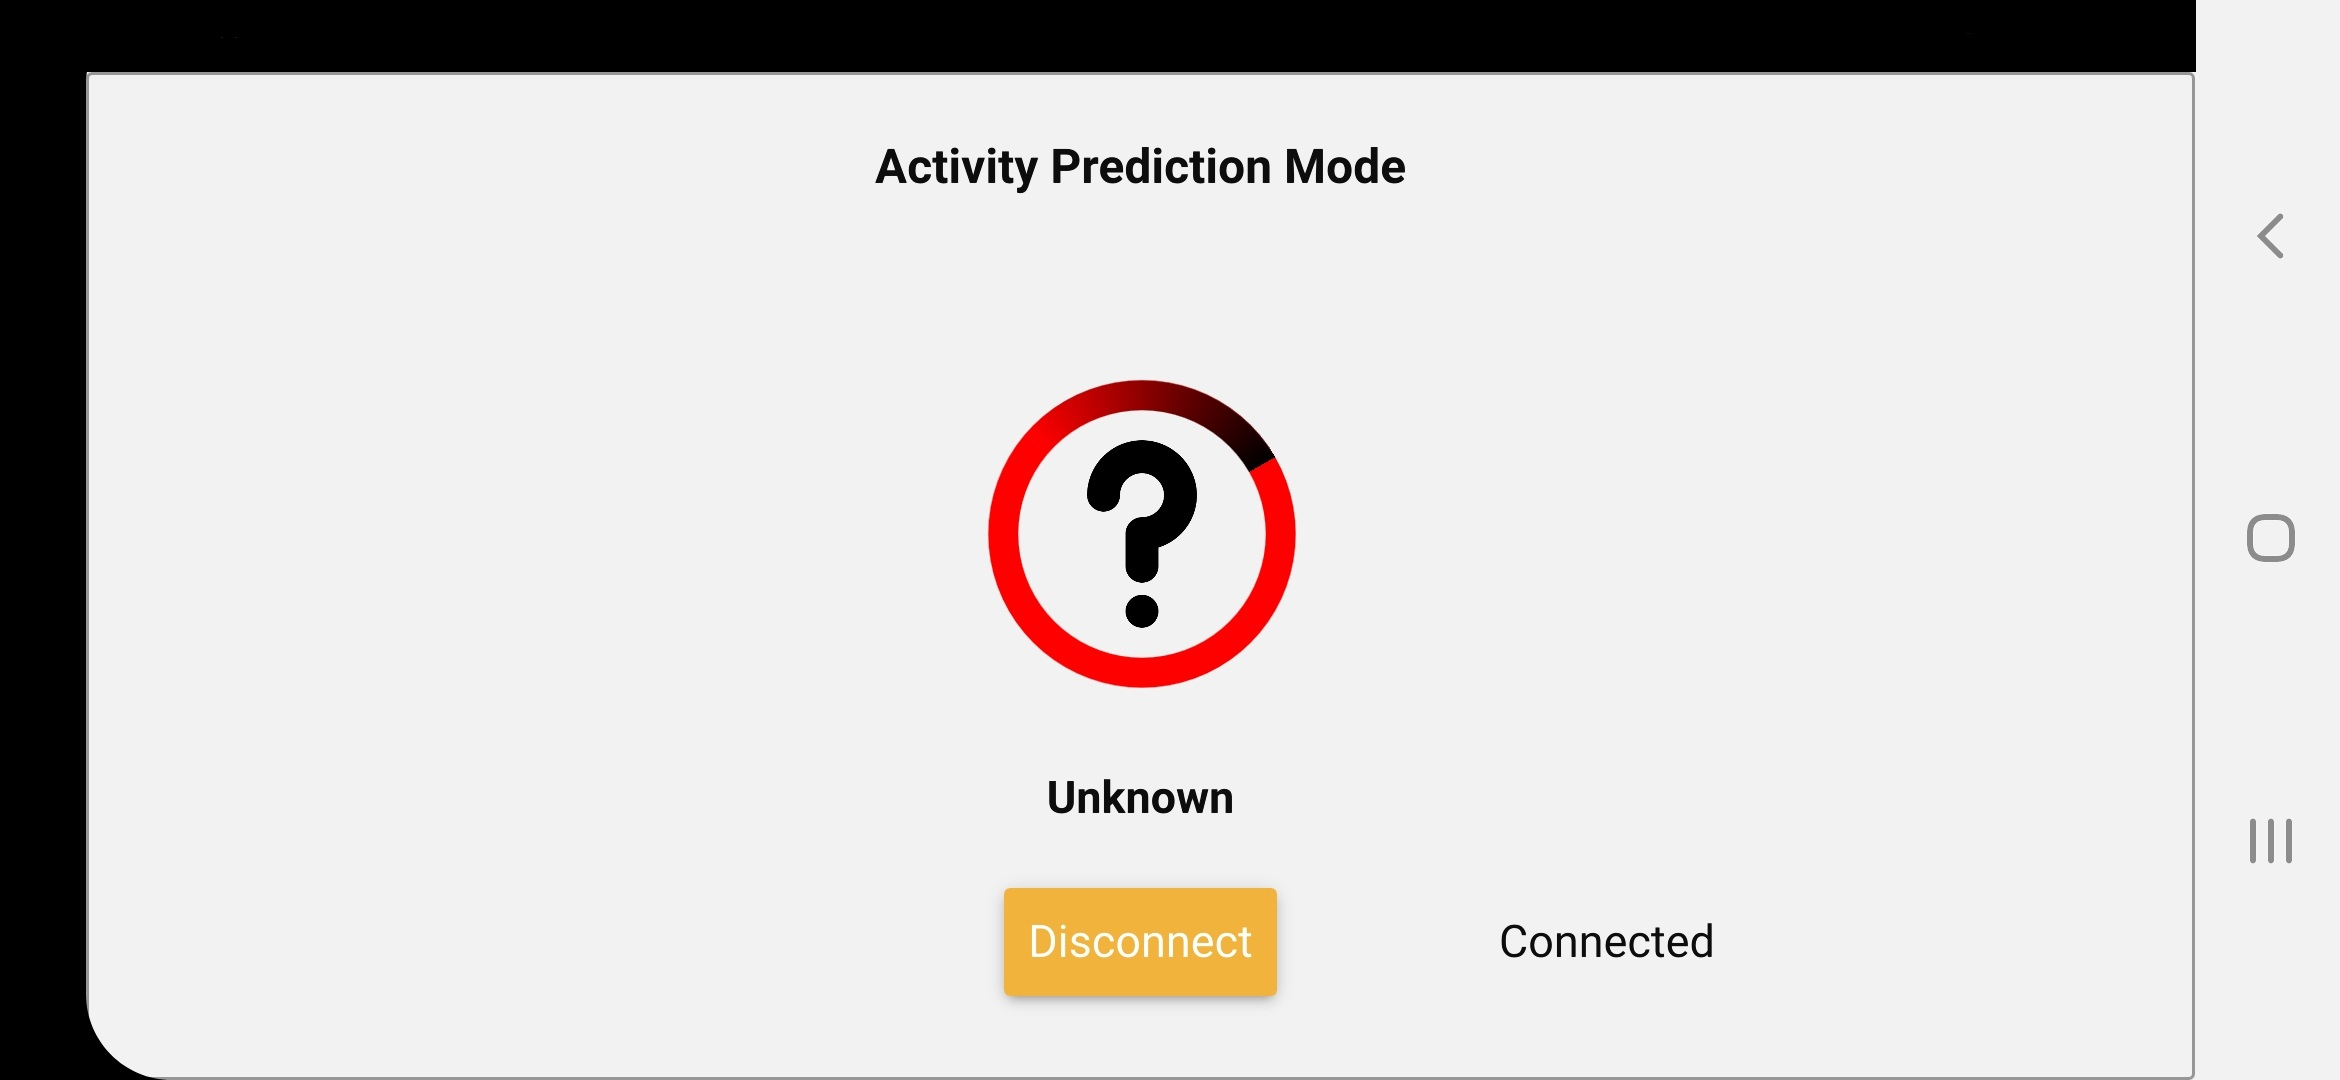
\includegraphics[width=0.4\linewidth]{./ImageFiles/unknown}
	\caption{Schermata per le attese precedenti la classificazione o per misure non classificabili.}
	\label{fig:attesa}
\end{figure}